\documentclass[11pt]{article}
\usepackage[scaled=0.92]{helvet}
\usepackage{geometry}
\geometry{letterpaper,tmargin=1in,bmargin=1in,lmargin=1in,rmargin=1in}
\usepackage[parfill]{parskip} % Activate to begin paragraphs with an empty line rather than an indent %\usepackage{graphicx}
\usepackage{amsmath,amssymb, mathrsfs,  mathtools, dsfont}
\usepackage{tabularx}
\usepackage{tikz-cd}
\usepackage[font=footnotesize,labelfont=bf]{caption}
\usepackage{graphicx}
\usepackage{xcolor}
%\usepackage[linkbordercolor ={1 1 1} ]{hyperref}
%\usepackage[sf]{titlesec}
\usepackage{natbib}
%\usepackage{tikz-cd}

\usepackage{../../Tianpei_Report}

%\usepackage{appendix}
%\usepackage{algorithm}
%\usepackage{algorithmic}

%\renewcommand{\algorithmicrequire}{\textbf{Input:}}
%\renewcommand{\algorithmicensure}{\textbf{Output:}}



\begin{document}
\title{Lecture 5: Concentration of Measure and Isoperimetry}
\author{ Tianpei Xie}
\date{Jan. 19th., 2023 }
\maketitle
\tableofcontents
\newpage
\section{The Classic Isoperimetry Inequalities}
\subsection{Brunn-Minkowski Inequality}
\begin{itemize}
\item \begin{definition} (\textbf{\emph{Minkowski Sum of Sets}})\\
Consider sets $A, B \subseteq \bR^n$ and define \underline{\emph{\textbf{the Minkowski sum}}} of $A$ and $B$ as the set of all vectors in $\bR^n$ formed by sums of elements of $A$ and $B$:
\begin{align*}
A + B &:= \set{x+y: x \in A, y \in B}
\end{align*} 
Similarly, for $c \in \bR$, let $c A = \set{cx : x \in A}$. Denote by $\text{Vol}(A)$ the \emph{\textbf{Lebesgue measure}} of a \emph{(measurable) set $A \subset \bR^n$}.
\end{definition}


\item \begin{theorem} (\textbf{Brunn-Minkowski Inequality}) \citep{boucheron2013concentration, vershynin2018high, wainwright2019high}\\
Let $A, B \subset \bR^n$ be \textbf{non-empty compact sets}. Then for all $\lambda \in [0, 1]$,
\begin{align}
\text{Vol}\paren{ \lambda A + (1- \lambda) B }^{\frac{1}{n}} &\ge \lambda\text{Vol}(A)^{\frac{1}{n}} + (1- \lambda)\text{Vol}(B)^{\frac{1}{n}}.   \label{ineqn: brunn_minkowski_inequality}
\end{align}
\end{theorem}
Note:  a convex body in $\bR^n$ is closed and compact set.
\begin{proof} (\textbf{\emph{Part 1, $n = 1$}})\\
Note that if $A \subset \bR$, and $c \ge 0$ then $\text{Vol}(cA) = c\text{Vol}(A)$. Thus it suffice to prove
\begin{align*}
\text{Vol}\paren{  A + B } &\ge \text{Vol}(A) + \text{Vol}(B).
\end{align*} To see this, observe that none of the three volumes involved changes if the sets $A$ and $B$ are \emph{\textbf{translated}} arbitrarily. Since $A, B$ are compact subsets in $\bR$, it is closed and bounded. Let $a = \max\{a': a' \in A\}$ and $b = \min\set{b': b' \in B}$. Let $A' = A +\set{-a}$ and $B' = B + \set{-b}$ so that $A' \subset (-\infty, 0]$ and $B' \subset [0, +\infty)$. Also $\text{Vol}(A') = \text{Vol}(A)$ and $\text{Vol}(B') = \text{Vol}(B)$. 
However, 
\begin{align*}
A' \cup B' &\subset A' + B' \\
\Rightarrow \text{Vol}(A') + \text{Vol}(B') = \text{Vol}(A' \cup B' ) &\le \text{Vol}(A' + B')
\end{align*} This prove the $1$-dimensional case for \emph{the Brunn-Minkowski inequality}. \qed

To prove $n > 1$ case, we need the following inequalities: 
\end{proof}

\item \begin{theorem} (\textbf{The Pr{\'e}kopa-Leindler Inequality}). \citep{boucheron2013concentration, wainwright2019high} \\
Let $\lambda \in (0, 1)$, and let $f, g, h : \bR^n \to [0, \infty)$ be \textbf{non-negative measurable functions} such that for all $x, y \in \bR^n$,
\begin{align*}
h\paren{\lambda x + (1- \lambda) y} &\ge f(x)^{\lambda}g(y)^{1-\lambda}.
\end{align*} Then
\begin{align}
\int_{\bR^n} h(x) dx &\ge \paren{\int_{\bR^n} f(x) dx }^{\lambda}\paren{\int_{\bR^n} g(x) dx}^{1-\lambda}.   \label{ineqn: prekopa_leindler_inequality}
\end{align}
\end{theorem}
\begin{proof}
The proof goes by induction with respect to the dimension $n$.
\begin{enumerate}
\item (\textbf{\emph{$n=1$ case}}). Consider measurable non-negative functions $f, g, h$ satisfying the condition of the theorem. By \emph{the monotone convergence theorem}, it suffices to prove the statement for \emph{\textbf{bounded functions}} $f$ and $g$.  Without loss of generality, assume that  $\sup_{x\in \bR^n} f(x) = \sup_{x\in \bR^n} g(x) = 1$.  Then
\begin{align*}
\int_{\bR} f(x) dx &= \int_{0}^{1}\text{Vol}\set{x: f(x) \ge t} dt \\
\int_{\bR} g(x) dx &= \int_{0}^{1}\text{Vol}\set{x: g(x) \ge t} dt.
\end{align*} For any fixed $t \in [0, 1]$, if $f(x) \ge t$ and $g(y) \ge t$, then by the hypothesis of the theorem, $h\paren{\lambda x + (1- \lambda) y} \ge t$. This implication may be re-written as
\begin{align*}
\lambda\set{x: f(x) \ge t} + (1- \lambda) \set{x: g(x) \ge t} &\subset \set{x: h(x) \ge t}.
\end{align*} Thus
\begin{align*}
\int_{\bR} h(x) dx &= \int_{0}^{\infty}\text{Vol}\set{x: h(x) \ge t} dt \\
&\ge  \int_{0}^{1}\text{Vol}\set{x: h(x) \ge t} dt \\
&\ge \int_{0}^{1} \text{Vol}\paren{\lambda\set{x: f(x) \ge t}} + \text{Vol}\paren{(1- \lambda) \set{x: g(x) \ge t}} dt \\
& (\text{ by $1$-dimensional \emph{Brunn-Minkowski inequality}}) \\
&\ge \lambda \int_{0}^{1}\text{Vol}\paren{\set{x: f(x) \ge t}}dt + (1- \lambda)\int_{0}^{1}\text{Vol}\paren{ \set{x: g(x) \ge t}}dt \\
& =\lambda   \int_{\bR} f(x) dx  + (1- \lambda) \int_{\bR} g(x) dx \\
&\ge \paren{\int_{\bR} f(x) dx }^{\lambda}\paren{\int_{\bR} g(x) dx}^{1-\lambda} \; \text{(by the \emph{arithmetic-geometric mean inequality})}
\end{align*}

\item For the induction step, assume that the theorem holds for all dimensions $1 \xdotx{,} n - 1$ and let $f, g, h : \bR^n \to [0, \infty)$,  $\lambda \in (0, 1)$ be such that they satisfy the assumption of the theorem.  Now let $x, y \in \bR^{n-1}$ and $a, b \in \bR$. Then
\begin{align*}
h\paren{\lambda \paren{x, a} + (1-\lambda)\paren{y, b}} \ge f\paren{(x, a)}^{\lambda} g((y, b))^{1- \lambda}, 
\end{align*} so by the inductive hypothesis
\begin{align*}
\int_{\bR^{n-1}} h\paren{(x, \lambda a + (1-\lambda) b)} dx &\ge \paren{\int_{\bR^{n-1}} f\paren{(x, a)} dx}^{\lambda}\paren{\int_{\bR^{n-1}} g((x, b)) dx }^{1- \lambda} 
\end{align*} In other words, introducing
\begin{align*}
F(a) := \int_{\bR^{n-1}} f\paren{(x, a)} dx, \quad G(b) := \int_{\bR^{n-1}} g((x, b)) dx\\
H((\lambda a + (1-\lambda) b)) := \int_{\bR^{n-1}} h\paren{(x, \lambda a + (1-\lambda) b)} dx.
\end{align*} We have
\begin{align*}
H((\lambda a + (1-\lambda) b))  &\ge \paren{F(a)}^{\lambda}\paren{G(b)}^{1- \lambda},
\end{align*} so by \emph{Fubini's theorem} and the one-dimensional inequality, we have
\begin{align*}
\int_{\bR^n}h(x) dx =  \int_{\bR} H(a)   da &\ge \paren{\int_{\bR} F(a) da}^{\lambda}\paren{\int_{\bR} G(a) da}^{1 - \lambda} \\
&= \paren{\int_{\bR^n} f(x) dx}^{\lambda}\paren{\int_{\bR^n} g(x) dx}^{1 - \lambda}.  \qed
\end{align*}
\end{enumerate} 
\end{proof}

\item \begin{corollary} (\textbf{Weaker Brunn-Minkowski Inequality}) \citep{boucheron2013concentration, wainwright2019high}\\
Let $A, B \subset \bR^n$ be \textbf{non-empty compact sets}. Then for all $\lambda \in [0, 1]$,
\begin{align}
\text{Vol}\paren{ \lambda A + (1- \lambda) B } &\ge \text{Vol}(A)^{\lambda}\text{Vol}(B)^{1- \lambda}.   \label{ineqn: brunn_minkowski_inequality_weaker}
\end{align}
\end{corollary}
\begin{proof}
We apply \emph{the Pr{\'e}kopa-Leindler inequality} with $f(x) = \ind{x \in A}$, $g(x) = \ind{x \in B}$ and $h(x) = \ind{x \in \lambda A + (1- \lambda) B}$. We see that 
\begin{align*}
h(\lambda x + (1- \lambda) y) &= \ind{\lambda x + (1- \lambda) y \in \lambda A + (1- \lambda) B} \ge \ind{x \in A, y \in B}  = f(x)^{\lambda}g(y)^{1 - \lambda}.
\end{align*} Thus the hypothesis of \emph{the Pr{\'e}kopa-Leindler inequality} holds. \qed
\end{proof}

\item \begin{proof}  (\textbf{\emph{$n> 1$ case for Brunn-Minkowski Inequality}}).  First observe that it suffices to prove that for all \emph{nonempty compact sets} $A$ and $B$,
\begin{align*}
\text{Vol}\paren{ A + B }^{\frac{1}{n}} &\ge \text{Vol}(A)^{\frac{1}{n}} + \text{Vol}(B)^{\frac{1}{n}}
\end{align*} since $\text{Vol}\paren{c A}^{1/n} = c \text{Vol}\paren{A}^{1/n}$ for any $c \in \bR$ and $A \subset \bR^n$. Also notice that we may assume that $ \text{Vol}(A),  \text{Vol}(B) > 0$ because otherwise the inequality holds trivially. Defining $A' = \text{Vol}(A)^{-\frac{1}{n}} A$ and $B' =  \text{Vol}(B)^{-\frac{1}{n}}B$, we have $ \text{Vol}(A') = \text{Vol}(B') = 1$. By \emph{weaker Brunn-Minkowski inequality}, for $\lambda \in (0, 1)$,
\begin{align*}
\text{Vol}\paren{ \lambda A' + (1- \lambda) B' } &\ge 1.
\end{align*} Finally, we apply this \emph{inequality} with the choice
\begin{align*}
\lambda &= \frac{\text{Vol}(A)^{\frac{1}{n}}}{\text{Vol}(A)^{\frac{1}{n}} + \text{Vol}(B)^{\frac{1}{n}}}
\end{align*} obtaining
\begin{align*}
\text{Vol}\paren{ \frac{\text{Vol}(A)^{\frac{1}{n}}A'}{\text{Vol}(A)^{\frac{1}{n}} + \text{Vol}(B)^{\frac{1}{n}}}  + \frac{\text{Vol}(B)^{\frac{1}{n}}B'}{\text{Vol}(A)^{\frac{1}{n}} + \text{Vol}(B)^{\frac{1}{n}}}  }  &\ge 1\\
\Rightarrow \text{Vol}\paren{ \frac{A}{\text{Vol}(A)^{\frac{1}{n}} + \text{Vol}(B)^{\frac{1}{n}}}  + \frac{B}{\text{Vol}(A)^{\frac{1}{n}} + \text{Vol}(B)^{\frac{1}{n}}}  }  &\ge 1 \\
\Rightarrow \text{Vol}\paren{ \frac{A + B}{\text{Vol}(A)^{\frac{1}{n}} + \text{Vol}(B)^{\frac{1}{n}}}    }  &\ge 1 \\
\Rightarrow \frac{\text{Vol}(A + B)}{\paren{\text{Vol}(A)^{\frac{1}{n}} + \text{Vol}(B)^{\frac{1}{n}}}^n} &\ge 1 
\end{align*} which proves the theorem. \qed
\end{proof}
\end{itemize}

\subsection{The Blowup of Sets and Classical Isoperimetry Theorem}
\begin{itemize}
\item \begin{definition} (\textbf{\emph{Blowup of Sets}}) \\
For any $t > 0$, and any (measurable) sets $A \subset \bR^n$,  \emph{\underline{\textbf{the $t$-blowup (or, $t$-enlargement)}} of $A$} is defined by
\begin{align*}
A_t &:= \set{x \in \bR^n: d(x, A) < t} = A + t\,B
\end{align*} where $B = \set{x \in \bR^n: d(0, x) < 1}$ is an \emph{open unit ball} and $d(x, A) = \inf_{y \in A}d(x, y)$.
\end{definition}

\item \begin{definition}(\textbf{\emph{Surface Area of Sets}}) \\
let $A \subset \bR^n$ be a measurable set and denote by $\text{Vol}(A)$ its \emph{Lebesgue measure}. \emph{The  \underline{\textbf{surface area}} of $A$} is
defined by
\begin{align*}
\text{Vol}(\partial A) &= \lim\limits_{t \to 0}\frac{\text{Vol}(A_t) - \text{Vol}(A)}{t}.
\end{align*} provided that the limit exists. Here $A_t$ denotes \emph{the $t$-blowup} of $A$.
\end{definition}

\item \begin{remark}(\textbf{\emph{Isoperimetry Theorem}})\\
The classical isoperimetric theorem in $\bR^n$ states that, among all sets with \emph{\textbf{a given volume}}, \underline{\emph{\textbf{the Euclidean unit ball minimizes the surface area}}}.  This theoerm can be formally stated as below:
\end{remark}

\begin{figure}
\begin{minipage}[t]{1\linewidth}
  \centering
  \centerline{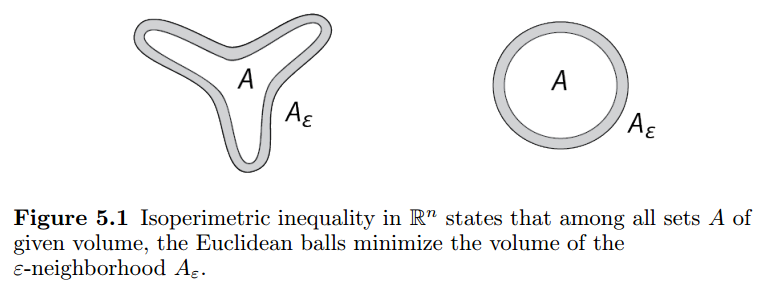
\includegraphics[scale = 0.4]{isoperimetry_rn.png}}
\end{minipage}
\caption{\footnotesize{\textbf{Isoperimetry in $\bR^{n}$  \citep{vershynin2018high}}}}
\label{fig: isoperimetry_rn}
\end{figure}


\item \begin{theorem} (\textbf{Isoperimetry Theorem}) \citep{boucheron2013concentration, vershynin2018high, wainwright2019high}\\
Let $A \subset \bR^n$ be such that $\text{Vol}(A) = \text{Vol}(B)$ where $B := \set{x \in \bR^n: d(0, x) < 1}$ is an unit ball. Then for any $t > 0$, 
\begin{align}
\text{Vol}(A_t) &\ge  \text{Vol}(B_t) \label{ineqn: isoperimetry_inequality_blowup}
\end{align} Moreover, if $\text{Vol}(\partial A) $ exists, then
\begin{align}
\text{Vol}(\partial A)  &\ge \text{Vol}(\partial B).  \label{ineqn: isoperimetry_inequality_surface}
\end{align}
\end{theorem}
\begin{proof}
By \emph{the Brunn-Minkowski inequality}, 
\begin{align*}
\text{Vol}(A_t)^{1/n}  = \text{Vol}(A + tB)^{1/n} &\ge \text{Vol}(A)^{1/n} +  t\text{Vol}(B)^{1/n} \\
&= (1+t) \text{Vol}(B)^{1/n} \\
&= \text{Vol}(B_t)^{1/n},
\end{align*} establishing the first statement. The second follows simply because
\begin{align*}
\text{Vol}(A_t) - \text{Vol}(A) &\ge \text{Vol}(B)((1+t)^n -1) \ge nt\text{Vol}(B)
\end{align*} where $(1+t)^n \ge 1 + nt$ for $t \ge 0$. Thus $\text{Vol}(\partial A)  \ge n\text{Vol}(B)$. The isoperimetric theorem now follows from the fact that
$\text{Vol}(\partial B) = n\text{Vol}(B)$. \qed
\end{proof}
\end{itemize}

\section{Concentration via Isoperimetry}
\subsection{Levy's Inequalities}
\begin{itemize}
\item \begin{remark}
We can generalize the classical isoperimety problem to a probability space $(\cX, \cB[\cX], \bP)$ where $\cX$ is a \emph{metric space} with metric $d$, $\cB[\cX]$ is the Borel $\sigma$-algrebra and $\bP$ is a probability measure on $\cB[\cX]$. Let  $B := \set{x \in \bR^n: d(0, x) < 1}$. The classical isoperimetry problem aims at finding the set $A^{*} \subset \cX$ that \emph{\textbf{minimizes the surface area}}
\begin{align*}
\bP(\partial A) = \lim\limits_{t \to 0}\frac{\bP(A_t) - \bP(A)}{t}
\end{align*} This is equivalent to find subset $A$ in $\cX$ with \emph{\textbf{minimal $t$-blowup}} for given $p$, and for all $t >0$
\begin{align*}
A^{*} := \inf_{A \subset \cX: \bP(A) \ge p}\bP(A_t), \quad \forall t > 0
\end{align*} where 
\begin{align*}
A_t = A + tB = \set{x \in \cX:  \exists y \in A \text{ s.t. } d(x, y) < t} = \set{x \in \cX:  \inf_{y \in A}d(x, y) := d(x, A) < t}.
\end{align*} We write the definition formally.
\end{remark}


\item \begin{definition} (\emph{\textbf{Isoperimetry Problem}}) \citep{boucheron2013concentration}\\
Given a \emph{\textbf{metric space}} $\cX$ with corresponding \emph{distance} $d$, consider \emph{\textbf{the measure space}} formed by $\cX$ , \emph{the $\sigma$-algebra} of all \emph{\textbf{Borel sets} of $\cX$}, and a probability measure $\bP$. Let $X$ be a \emph{random variable} taking values in $\cX$, distributed according to $\bP$. 

\underline{\emph{\textbf{The isoperimetric problem}}} in this case is the following: given $p \in (0, 1)$ and $t > 0$, \emph{\textbf{determine the sets}} $A$ with $\bP\brac{X \in A} \ge p$ for which \emph{the measure}
\begin{align*}
\bP\brac{d(X, A) \ge t}
\end{align*}  is \emph{\textbf{maximal}}. 
\end{definition}

\item \begin{remark} (\emph{\textbf{Isoperimetric Inequalities}})\\
Even though the exact solution is only known in a few special cases, useful \emph{bounds} for $\bP\brac{d(X, A) \ge t}$ can be derived under remarkably general circumstances. \emph{Such bounds are usually referred to as} \underline{\emph{\textbf{isoperimetric inequalities}}}.
\end{remark}

\item \begin{definition} (\textbf{\emph{Concentration Function}}) \citep{boucheron2013concentration, wainwright2019high}\\
\underline{\emph{\textbf{The concentration function}}} $\alpha: [0, \infty) \to \bR_{+}$  associated with \emph{\textbf{metric measure space}} $((\cX, d), \bP)$ is given by
\begin{align*}
\alpha_{\bP, (\cX, d)}(t) &:= \sup_{ A \subset \cX:\, \bP\paren{A} \ge \frac{1}{2}}\bP\brac{d(X, A) \ge t } = \sup_{A \subset \cX: \,\bP\paren{A} \ge \frac{1}{2}}\bP\paren{A_{t}^{c} }
\end{align*} where $A_t:= A + tB = \set{x \in \cX: d(x, A) < t}$ is \emph{the $t$-blowup} of $A \subset \cX$. We simply denote it as $\alpha(t)$.
\end{definition}
Thus the optimal $A^{*}$ for isoperimetry problem is the one that attains the $\alpha(t) = \bP\paren{A_{t}^{c} }$.

\item \begin{example} (\textbf{\emph{Concentration Function of Lebesgue Measure in $\bR^n$ and Isoperimetric Inequality}})\\
Note that the volume of a \emph{$t$-ball in $\bR^n$} is 
\begin{align*}
\text{Vol}(tB) =  \frac{\pi^{\frac{n}{2}}}{\Gamma\paren{\frac{n}{2} + 1}}t^n  \equiv c_n t^n 
\end{align*}  Thus the radius of ball $B$ with the same volume of $A$ is
\begin{align*}
r := \paren{\frac{\text{Vol}(A) }{c_n}}^{\frac{1}{n}}.
\end{align*} \emph{\textbf{The classical isoperimetric inequality}} states that 
\begin{align}
 \text{Vol}(A_t)) &\ge \paren{ (r+  t)\text{Vol}(B)^{1/n}}^{n} \nonumber\\
 \Leftrightarrow  \text{Vol}(A_t) &\ge c_n\paren{\paren{\frac{\text{Vol}(A) }{c_n}}^{\frac{1}{n}} + t}^n \nonumber \\
  \Leftrightarrow  \paren{\frac{\text{Vol}(A_t) }{c_n}}^{\frac{1}{n}}  &\ge \paren{\frac{\text{Vol}(A) }{c_n}}^{\frac{1}{n}} + t  \label{ineqn: lebesgure_measure_concentration}
\end{align} Define  \emph{\textbf{the isoperimetric function}} of \emph{the Lebesgue measure space} $(\bR^n, \mu)$ as
\begin{align*}
\lambda(u) := \paren{\frac{u}{c_n}}^{\frac{1}{n}}
\end{align*} so \emph{the classical isoperimetric inequality}  is equivalent to \emph{the concentration of Lebesgue measure}
\begin{align*}
\lambda\paren{\mu(A_t)} &\ge \lambda\paren{\mu(A)} + t. 
\end{align*}
\end{example}

\item \begin{theorem} (\textbf{Levy's Inequalities})\citep{boucheron2013concentration, wainwright2019high}\\
For any Lipschitz function $f: \cX \to \bR$, 
\begin{align}
\bP\set{f(X) \ge  \text{Med}(f(X)) + t } &\le \alpha_{\bP}(t) \label{ineqn: levy_inequality}\\
\bP\set{f(X)  \le  \text{Med}(f(X))  -  t } &\le \alpha_{\bP}(t).  \nonumber
\end{align} where $\text{Med}(f(X))$ is \underline{\textbf{the median} of $f(X)$}, i.e.
\begin{align*}
\bP\set{f(X) \le \text{Med}(f(X)} \ge  \frac{1}{2}, \;\text{ and }\; \bP\set{f(X) \ge \text{Med}(f(X)} \ge  \frac{1}{2}.
\end{align*}
\end{theorem}
\begin{proof} 
Consider the set $A = \set{x : f(x) \le \text{Med}(f(X))}$. By the definition of a \emph{median},  $\bP\paren{A} \ge \frac{1}{2}$. On the other hand, by \emph{the Lipschitz property} of $f$, for any $x, y \in \cX$,
\begin{align*}
\abs{f(x) - f(y)} \le d(x, y). 
\end{align*} So for all $y \in A$,  $f(y) \le \text{Med}(f(X))$
\begin{align*}
f(x) -  \text{Med}(f(X))  &\le f(x) - f(y) \le d(x, y) \\
\Rightarrow  f(x) -  \text{Med}(f(X))  &\le \inf_{y \in A}d(x, y) := d(x, A).
\end{align*} Equivalently, 
\begin{align*}
A_t := \set{x \in \cX: d(x, A) < t} &\subseteq \set{x \in \cX:  f(x) < \text{Med}(f(X)) + t } \\
\bP(A_t^{c}) &\ge \bP\set{ f(X) \ge \text{Med}(f(X)) + t } 
\end{align*} The first inequality now follows from the definition of the concentration function.  The second inequality follows from the first by considering $–f$.  \qed
\end{proof}

\item \begin{remark} For $L$-Lipschitz function $f$, the inequality becomes
\begin{align*}
\bP\set{f(X) - \text{Med}(f(X)) \ge t } \le  \alpha\paren{\frac{t}{L}}, \quad \bP\set{f(X) - \text{Med}(f(X)) \le -t } &\le \alpha\paren{\frac{t}{L}}.
\end{align*}
\end{remark}

\item \begin{theorem}  (\textbf{Converse of Levy's Inequalities})\citep{boucheron2013concentration, wainwright2019high}\\
If $\beta : \bR_{+} \to [0, 1]$ is a function such that for \textbf{every Lipschitz function} $f : \cX \to \bR$
\begin{align}
\bP\set{f(X) - \text{Med}(f(X)) \ge t } &\le \beta(t). \label{ineqn: converse_levy_inequality}
\end{align} then $\beta(t) \ge \alpha_{\bP}(t)$.
\end{theorem}
\begin{proof}
Note that for any $A \subset \cX$ , the function $f_A$ defined by $f_A(x)= d(x, A)$ is \emph{Lipschitz} since
\begin{align*}
\abs{f_A(x) - f_A(y)} = \abs{d(x, A) - d(y, A)} &\le d(x, y).
\end{align*} Also, if  $P\paren{A} \ge 1/2$, then $0$ is a median of $f_A(X)$, since
\begin{align*}
\bP\set{f_A(x) \le 0} = \bP\set{d(X, A) \le 0} = \bP(A) \ge \frac{1}{2}.
\end{align*}  Therefore
\begin{align*}
\alpha(t) := \sup_{A \subset \cX: \bP(A) \ge 1/2}\bP\set{f_A(x) - \text{Med}(f_A(X)) \ge t} \le \beta(t). \qed
\end{align*}
\end{proof}

\item \begin{proposition} (\textbf{Levy's Inequalities for Mean})\citep{boucheron2013concentration, wainwright2019high}\\
If $\beta: \bR_{+} \to [0,1]$ is a  function such that for \textbf{every Lipschitz function} $f : \cX \to \bR$
\begin{align}
\bP\set{f(X) - \E{}{f(X)} \ge t } &\le \beta(t). \label{ineqn: converse_levy_inequality_mean}
\end{align} then $\beta(t) \ge \alpha_{\bP}(t/2)$.
\end{proposition}

\item \begin{remark} (\emph{\textbf{Isoperimetric Inequalities $\Leftrightarrow$ Concentration of Lipschitz Functions}})\\
The first result points out that \emph{isoperimetric inequalities} (more precisely, \emph{\textbf{upper bounds} for \textbf{the concentration function}}) imply
\emph{concentration of Lipschitz functions}. 

\emph{\textbf{The converse}} shows that \emph{concentration of Lipschitz functions} implies an \emph{isoperimetric inequality}. In other word, \emph{among all upper bounds} of $\bP(A_t^c)$ for fixed $A_t$, 
\end{remark}

\item \begin{corollary} (\textbf{Concentration of  Measure on Hamming Metric Space}) \citep{boucheron2013concentration}\\
Consider \emph{independent random variables} $Z_1 \xdotx{,} Z_n$ taking their values in a \emph{(measurable) set} $\cX$ and denote the vector of these variables by $Z = (Z_1 \xdotx{,} Z_n)$ taking its value in $\cX^n$.  For an arbitrary (measurable) set $A \subset \cX^n$, we write $\bP\paren{A} = \bP\paren{Z \in A}$.  The \textbf{Hamming distance} $d_{H}(x, y)$ between the vectors $x, y \in \cX^n$ is defined as \textbf{the number of coordinates} in which $x$ and $y$ \textbf{differ}. Then for any $t >0$, 
\begin{align}
\bP\set{d_{H}(x, A) \ge \sqrt{\frac{n}{2}\log \frac{1}{\bP(A)}} + t} \le \exp\paren{-\frac{2t^2}{n}}  \label{ineqn: isoperimetry_inequality_hamming_distance}
\end{align}
\end{corollary}
\begin{proof}
As we shown in previous proof, $f_A(x) = d_{H}(x, A)$ is a Lipschitz function with respect to Hamming distance $d_H$. It follows from the definition that 
\begin{align*}
\sup_{x \in \cX^n, y_i \in \cX}\abs{f_{A}(x) - f_{A}(\widetilde{x}^{(i)})} \le d_{H}(x, \widetilde{x}^{(i)}) = 1
\end{align*} where $\widetilde{x}^{(i)} = (x_1 \xdotx{,} x_{i-1}, y_i, x_{i+1} \xdotx{,} x_{n})$, so $f_A$ has the bounded difference property. By bounded difference inequality, 
\begin{align*}
\bP\set{ \E{}{f_{A}(Z)} - f_{A}(Z)  \ge t }  &\le \exp\paren{-\frac{2t^2}{n}}.
\end{align*} Taking $t = \E{}{f_{A}(Z)} = \E{}{d_{H}(Z, A)}$, the left-hand side becomes $\bP\set{f_{A}(Z) \le 0} = \bP\set{d_{H}(Z, A)  \le 0}  = \bP\paren{A}$. Then the inequality becomes
\begin{align*}
\bP\paren{A} &\le \exp\paren{- \frac{2}{n} \paren{\E{}{d_{H}(Z, A)}}^2} \\
\Rightarrow \E{}{d_{H}(Z, A)} &\le \sqrt{\frac{n}{2}\log \frac{1}{\bP(A)}}.
\end{align*} Then, by using the bounded difference inequality again, we obtain
\begin{align*}
\bP\set{d_H(Z, A) \ge  \sqrt{\frac{n}{2}\log \frac{1}{\bP(A)}} + t } \le \bP\set{d_H(Z, A) \ge  \E{}{d_{H}(Z, A)} + t } \le \exp\paren{-\frac{2t^2}{n}}. \qed
\end{align*}
\end{proof}

\item \begin{remark} (\textbf{\emph{Equivalent Form}})\\
From above isoperimetric inequality, 
\begin{align*}
\bP\set{d_{H}(x, A) \ge \sqrt{\frac{n}{2}\log \frac{1}{\bP(A)}} + t} \le \exp\paren{-\frac{2t^2}{n}}
\end{align*} Denote $u := \sqrt{\frac{n}{2}\log \frac{1}{\bP(A)}}$. By change of variable, for any $t \ge u$, 
\begin{align*}
\bP\set{d_{H}(x, A) \ge t} \le \exp\paren{-\frac{2\paren{t - u}^2}{n}}.
\end{align*} On the one hand, if $t \le 2u = \sqrt{-2 n \log \bP\paren{A}}$, then $\bP\paren{A} \le \exp(-t^2/(2n))$. On the other hand,
since $(t - u)^2 \ge t^2/4$ for $t \ge 2u =  \sqrt{-2 n \log \bP\paren{A}}$. the inequality above implies
$\bP\set{d_{H}(x, A) \ge t} \le  \exp(-t^2/(2n))$.
Thus, for all $t > 0$, we have \textbf{\emph{the concentration of measure in Hamming metric space}}:
\begin{align}
\bP(A)\bP\set{d_{H}(x, A) \ge t} \le \min\set{\bP(A), \bP\set{d_{H}(x, A) \ge t}} \le  \exp\paren{-\frac{t^2}{2n}} \label{ineqn: concentration_measure_hamming_distance}
\end{align}
\end{remark}


\item \begin{remark} (\textbf{\emph{Concentration of Measure}})\\
To interpret the result in \eqref{ineqn: isoperimetry_inequality_hamming_distance}, we see that on the left-hand side we have the measure of the set of points whose Hamming distance is at least $t + \sqrt{\frac{n}{2}\log \frac{1}{\bP(A)}}$ away from $A$. This inequality means that for $A$ with \emph{\textbf{small measure}} $\bP(A)$, the measure of points whose \emph{\textbf{Hamming distance}} from $A$ \emph{is less than} $O\paren{\sqrt{n}}$ is \emph{\textbf{extremely large}}.
In other words, \emph{\textbf{product measure} on Hamming metric space are \textbf{concentrated} on \textbf{extremely small sets}}. This phenonemon is called ``\underline{\textbf{\emph{concentration of measure}}}". 
\end{remark}

\item \begin{example} (\textbf{\emph{Bounded Difference Property $\Leftrightarrow$ Lipschitz Condition w.r.t. Hamming Distance}}) \\
Note that any  function with \emph{\textbf{bounded difference property}} is \emph{\textbf{Lipschitz function}} with respect to \emph{\textbf{Hamming distance}}. 
\begin{align*}
&\sup_{x \in \cX^n, y_i \in \cX}\abs{f(x_1 \xdotx{,} x_n) - f(x_1 \xdotx{,} x_{i-1}, y_i, x_{i+1} \xdotx{,} x_{n})} &\\
&\le c_i = c_i\,d_{H}((x_1 \xdotx{,} x_n), (x_1 \xdotx{,} x_{i-1}, y_i, x_{i+1} \xdotx{,} x_{n})), \quad 1\le i \le n\\
\Rightarrow \abs{f(x) - f(y)} &=  \abs{\sum_{i=1}^{n}(f(x_{(i-1)}) - f(x_{(i)}) )}\\
&\quad \le  \sum_{i=1}^{n}\abs{f(x_{(i-1)}) - f(x_{(i)}) }\\
&\quad \le \sum_{i=1}^{n}c_i \ind{x_{(i-1)}[i] \neq x_{(i)}[i]} \\
&\quad = d_{H,c}(x, y)
\end{align*}   where $x_{(i)}$ is replicate of $x_{(i-1)}$ except for $i$-th component, which is replaced by $y_i$. Note that $x_{(0)} = x$ and $x_{(n)} = y$. 
Therefore, \emph{the bounded difference inequality} can be seen as \emph{an isoperimetry inequality} for \emph{Lipschitz function with respect to Hamming distance}.
\begin{align*}
 \bP\set{f(Z) - \E{}{f(Z)} \ge t } &\le \exp\paren{-\frac{2t^2}{n}}
\end{align*}
\end{example}


\end{itemize}
\subsection{Isoperimetric Inequalities on the Unit Sphere}
\begin{itemize}
%\item \begin{remark} (\emph{\textbf{Volume Ratio of Unit Balls and its Interior}})  \citep{vershynin2018high}\\
%Let $B(0, 1):= \set{x \in \bR^n: \norm{x}{} \le 1}$ be the unit ball in $\bR^n$. The volume ratio between $B(0,1)$ and its $\epsilon$-interior $B(0, 1-\epsilon)$ is
%\begin{align*}
%\frac{\text{Vol}(B(0, 1-\epsilon))}{\text{Vol}(B(0,1))} &= (1 - \epsilon)^n \le \exp\paren{-n \epsilon}
%\end{align*} The inequality is due to $1 - x\le e^{-x}$.  
%
%As $n \to \infty$, the above ratio goes to $0$. In other words, most of volume in $B(0,1)$ is \emph{\textbf{concentrated}} in the \emph{\textbf{boundary}} $\partial B = \bS^{n-1} := \set{x \in \bR^n: \norm{x}{} = 1}$. This phenomenon is called ``\emph{\textbf{the curse of dimensionality}}".
%\end{remark}
\begin{figure}
\begin{minipage}[t]{1\linewidth}
  \centering
  \centerline{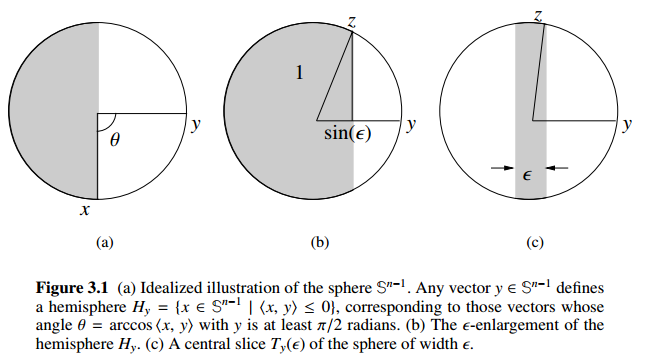
\includegraphics[scale = 0.5]{spherical_cap_blowup.png}}
\end{minipage}
\caption{\footnotesize{\textbf{spherical cap and $t$-blowup.   \citep{wainwright2019high}}}}
\label{fig: spherical_cap_blowup}
\end{figure}


\item \begin{definition} (\textbf{\emph{Spherical Cap and its $t$-Blowup}}) \\
Let $\bS^{n - 1} :=  \set{x \in \bR^n: \norm{x}{} = 1}$ be the \emph{$(n-1)$-dimensional \textbf{unit sphere}}. The \emph{\textbf{intersection}} of a \emph{\textbf{half-space}} and $\bS^{n-1}$ is called a \emph{\textbf{spherical cap}}. In particular, for some $y \in \bR^n$, denote the associated spherical cap as
\begin{align*}
H_y := \set{x \in \bS^{n-1}: \inn{x}{y} \le 0}
\end{align*} With some simple geometry, it can be shown that its  \emph{$t$-blowup}  corresponds to the set
\begin{align*}
H_y^{t} := \set{x \in \bS^{n-1}: \inn{x}{y} < \sin(t)}
\end{align*}
\end{definition}

\item \begin{theorem} (\textbf{Isoperimetry Theorem on Unit Sphere}) \citep{boucheron2013concentration, vershynin2018high, wainwright2019high}\\
Let $A$ be a subset of the sphere $\bS^{n-1}$, and let $\sigma$ denote the \textbf{normalized area} on that sphere. Let $t > 0$. Then,
among all sets $A \subset \bS^{n-1}$ with given area $\sigma(A)$, the \underline{\textbf{spherical caps}} \textbf{minimize}
\textbf{the area of the neighborhood} $\sigma(A_t)$, where
\begin{align*}
A_t := \set{x \in \bS^{n-1}: \exists y \in A \text{ such that } \norm{x - y}{} < t}
\end{align*}
\end{theorem}

\item \begin{remark}
Define a \emph{metric} $\rho$ on sphere $\bS^{n-1}$ as 
\begin{align*}
\rho(x, y) := \arccos(\inn{x}{y})
\end{align*}
Thus $(\bS^{n-1}, \rho)$ is a \emph{\textbf{metric space}}.  Let $\bP$ be uniform distribution on $\bS^{n-1}$ so that $((\bS^{n-1}, \rho), \bP)$ is a probability space. 
\end{remark}



\item \begin{proposition} (\textbf{Isoperimetric Inequalities for Uniform Distribution over Sphere})  \citep{boucheron2013concentration, vershynin2018high, wainwright2019high}\\
Let $\bS^{n - 1} :=  \set{x \in \bR^n: \norm{x}{} = 1}$ be the $(n-1)$-dimensional \textbf{unit sphere}.  For any $t\in [0, 1]$, 
\begin{align}
\alpha_{\bS^{n-1}}(t) &\le c \exp\paren{-\frac{n t^2}{2}} \label{ineqn: isoperimetric_inequality_uniform_unit_sphere}
\end{align} for some constant $c$.
\end{proposition}
\begin{proof}
Consider spherical cap 
\begin{align*}
C(y, 0) := \set{x \in \bS^{n-1}: \inn{x}{y} \ge 0}
\end{align*} and its  \emph{$t$-blowup}
\begin{align*}
C(y, t) :=  \set{x \in \bS^{n-1}: \inn{x}{y} \ge t}.
\end{align*} According to \emph{the isoperimetry theorem on unit sphere}, the concentration function for uniform distribution over $\bS^{n-1}$
\begin{align*}
\alpha_{\bS^{n-1}}(t) &= \bP(C(y, t)).
\end{align*} 

\begin{figure}
\begin{minipage}[t]{0.5\linewidth}
  \centering
  \centerline{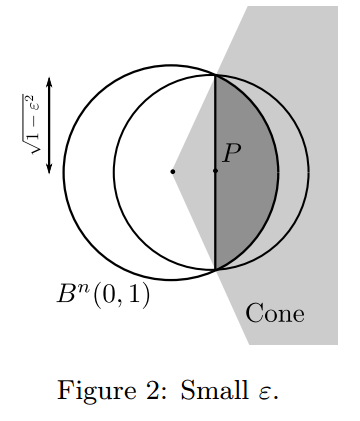
\includegraphics[scale = 0.4]{spherical_cap_proof.png}}
\end{minipage}
\begin{minipage}[t]{0.5\linewidth}
  \centering
  \centerline{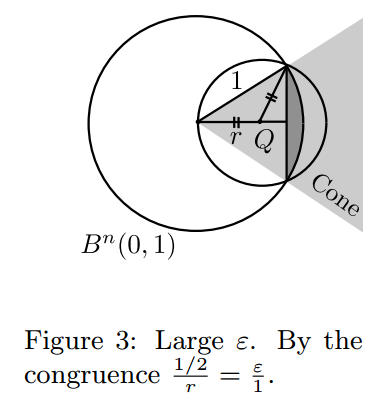
\includegraphics[scale = 0.4]{spherical_cap_proof_2.png}}
\end{minipage}
\caption{\footnotesize{\textbf{proof for upper bound of area of spherical cap (left) for small $t$ (right) for large $t$}}}
\label{fig: spherical_cap_blowup}
\end{figure}


Note that $\bP\paren{C(y, 0)} \le 1/2$.  In order to bound the concentration function from above, consider for small $t \in [0, 1/\sqrt{2}]$,
\begin{align*}
\alpha_{\bS^{n-1}}(t) = \bP\paren{C(y, t)} &= \frac{\text{Vol}(B^n(0, 1)\cap \text{Cone})}{\text{Vol}(B^{n}(0,1))} \\
&\le \frac{\text{Vol}(B^n(P,  \sqrt{1 - t^2}))}{\text{Vol}(B^{n}(0,1))}\\
&= (\sqrt{1 - t^2})^{n} \\
&\le \exp\paren{-  \frac{nt^2}{2}}
\end{align*}

For $t \in [1/\sqrt{2}, 1)$, it is enough to consider a different auxiliary ball which includes the set $\text{Cone} \cap B^n(0, 1)$. We obtain
\begin{align*}
\alpha_{\bS^{n-1}}(t) = \bP\paren{C(y, t)} & \le \frac{\text{Vol}(B^n(Q,  r))}{\text{Vol}(B^{n}(0,1))}\\
&= r^n = \paren{\frac{1}{2t}}^n\\
&\le \exp\paren{-\frac{n t^2}{2}}
\end{align*} where the last inequality is from $e^{x^2/2} \le 2x$ for $x \in [1/\sqrt{2}, 1]$. Due to convexity, this is only to be checked at the boundary of our interval
$[1/\sqrt{2}, 1]$,  \qed
%we see that $\sin(t) \ge t/2$ for $t \in (0, \pi/2]$. Then the $t$-blowup $H_y^{t}$ must contain set
%\begin{align*}
%\widetilde{H}_y^{t} := \set{x \in \bS^{n-1}: \inn{x}{y} < \frac{t}{2}},
%\end{align*} hence $\bP(\widetilde{H}_y^{t}) \le \bP(H_y^{t} )$. By geometric calculation, for all $t\in (0, \sqrt{2})$, we have 
%\begin{align*}
%\bP(\widetilde{H}_y^{t}) &\ge 1- \brac{1 - \paren{\frac{t}{2}}^2}^{n/2} \ge 1 - \exp\paren{-\frac{n\,t^2}{8}}
%\end{align*} where the last inequality is due to $(1 - x) \le e^{-x}$. Thus
%\begin{align*}
%\alpha_{\bS^{n-1}}(t) &= 1 - \bP(H_y^{t}) \le \exp\paren{-\frac{n\,t^2}{8}}.
%\end{align*} A similar but more careful approach to bounding $\bP(H_y)$ can be used to establish the sharper upper bound
%\begin{align*}
%\alpha_{\bS^{n-1}}(t) &\le  \sqrt{\frac{\pi}{2}}\exp\paren{-\frac{n t^2}{2}}. \qed
%\end{align*}
\end{proof}

\item By Levy's inequality, we have the following proposition
\begin{proposition} (\textbf{Lipschitz Function on $\bS^{n-1}$}) \citep{wainwright2019high}\\
For any $1$-Lipschitz function $f$ defined on the sphere $\bS^{n-1}$, we have the two-sided bound
\begin{align}
\bP\set{\abs{f(Z) - \text{Med}(f(Z))} \ge t} &\le \sqrt{2\pi}\exp\paren{-\frac{n t^2}{2}} \label{ineqn: lipschitz_unit_sphere_median}
\end{align} Moreover, replacing median by the mean, we have 
\begin{align}
\bP\set{\abs{f(Z) - \E{}{f(Z)} } \ge t} &\le 2\sqrt{2\pi}\exp\paren{-\frac{n t^2}{8}} \label{ineqn: lipschitz_unit_sphere_mean}
\end{align}
\end{proposition}

\item \begin{exercise} \textbf{(The Blow-Up Phenomenon)}\\
Let $A$ be a subset of the sphere $\sqrt{n} \bS^{n-1}$ such that
\begin{align*}
\bP\paren{A} > 2 \exp\paren{-c s^2} \text{ for some }s > 0;
\end{align*}
\begin{enumerate}
\item Prove that $\bP(A_s) > 1/2$.
\item Deduce from this that for any $t \ge s$,
\begin{align*}
\bP\paren{A_{2t}} > 1 - 2 \exp\paren{-c t^2}.
\end{align*} Here $c > 0$ is the absolute constant in upper bound of concentration function.
\end{enumerate}
\end{exercise}

\item \begin{remark} (\textbf{\emph{Zero-One Law for Independent Variables}}) \citep{vershynin2018high}\\
\emph{\textbf{The blow-up phenomenon}} we just saw may be quite \emph{counter-intuitive} at first sight. How can an exponentially small set $A$ undergo such a dramatic transition to an exponentially large set $A_{2t}$ under such a small perturbation $2t$ ? (Remember that $t$ can be much smaller than the radius $\sqrt{n}$ of the sphere.) 

However perplexing this may seem, this is \emph{a typical phenomenon in \textbf{high dimensions}}. It is \emph{reminiscent} of \textbf{\emph{zero-one laws}} in
\emph{probability theory}, which basically state that \emph{events that are determined by many random variables} tend to have \emph{probabilities either zero or one}.
\end{remark}
\end{itemize}
\subsection{Gaussian Isoperimetric Inequalities and  Concentration of Gaussian Measure}
\begin{itemize}
\item \begin{remark} (\textbf{\emph{Gaussian Isoperimetric Problem}})\\
\underline{\emph{\textbf{The Gaussian isoperimetric problem}}} is to determine which (Borel) sets $A$ have \emph{\textbf{minimal Gaussian boundary measure}} among all sets in $\bR^n$ with a \emph{given probability} $p$. 

\underline{\emph{\textbf{The Gaussian isoperimetric theorem}}} states the beautiful fact that \underline{\emph{\textbf{the extremal sets}}} are \underline{\emph{\textbf{linear half-spaces}}} \emph{in all dimensions} and \emph{for all $p$}.
\end{remark}

\item \begin{definition} (\textbf{\emph{Gaussian Isoperimetric Function}}) \\
Denote \emph{the cumulative distribution function of standard Normal distribution}:
\begin{align*}
\Phi(x) &= \int_{-\infty}^{x}\frac{1}{\sqrt{2\pi}}e^{-\frac{t^2}{2}}dt := \int_{-\infty}^{x}\varphi(t) dt
\end{align*} where $\varphi(x) := \frac{1}{\sqrt{2\pi}}e^{-\frac{t^2}{2}} = (\Phi(x))'$ is \emph{the probability density function} of standard normal distribution. $\Phi^{-1}(x)$ is \emph{the quantile function of normal distribution}.

Define \underline{\textbf{\emph{the Gaussian isoperimetric function}}} as 
\begin{align*}
\gamma(x) &:= \varphi\paren{\Phi^{-1}(x)}, \quad x \in (0,1). 
\end{align*} Also we define $\gamma(0) = \gamma(1) = 0$. 
\end{definition}

\item \begin{remark}
Note that
\begin{align*}
x &= \Phi(\Phi^{-1}(x)) \\
\Rightarrow 1 &= \varphi(\Phi^{-1}(x))(\Phi^{-1}(x))'  = \gamma(x) (\Phi^{-1}(x))' \\
\Leftrightarrow 1/\gamma(x) &= (\Phi^{-1}(x))'.
\end{align*} The quantity $1/\gamma(x) = (\Phi^{-1}(x))'$ is known as \emph{\textbf{quantile-density function} of normal distribution}.
\end{remark}

\item \begin{proposition}(\textbf{Basic Property of the Gaussian Isoperimetric Function}) \citep{boucheron2013concentration} \\
The Gaussian isoperimetric function $\gamma$ satisfies:
\begin{enumerate}
\item 
\begin{align*}
\gamma'(x) &= - \Phi^{-1}(x), \quad \text{ for all }x \in (0,1),
\end{align*}
\item 
\begin{align*}
\gamma(x)\gamma''(x) &= - 1, \quad \text{ for all }x \in (0,1),
\end{align*}
\item $(\gamma')^2$ is convex over $(0, 1).$
\end{enumerate}
\end{proposition}
\begin{proof}
\begin{enumerate}
\item See that
\begin{align*}
\varphi'(x) &= \frac{1}{\sqrt{2\pi}}(-x)e^{-\frac{x^2}{2}} = (-x)\varphi(x)\\
\varphi''(x) &= (x^2-1)\varphi(x)
\end{align*} Thus
\begin{align*}
\gamma(x)' &= (\varphi\paren{\Phi^{-1}(x)})^{'} = \frac{d\varphi}{dy}(\Phi^{-1}(x)) \frac{d\Phi^{-1}}{dx}(x) =(-\Phi^{-1}(x)) \paren{\Phi^{-1}(x)}'\gamma(x) = -\Phi^{-1}(x), 
\end{align*} since $\paren{\Phi^{-1}(x)}'\gamma(x) = 1$, we have the result. 

\item \begin{align*}
\gamma''(x) = (\gamma'(x))' &= -\paren{\Phi^{-1}(x)}' = - \frac{1}{\gamma(x)}\\
\gamma(x)\gamma''(x) &= -1
\end{align*}

\item Since $\gamma > 0$ for $x \in (0, 1)$, 
\begin{align*}
\gamma''(x) &= -\frac{1}{\gamma(x)} < 0.
\end{align*}  Thus $\gamma(x)$ is concave function  in $(0, 1)$. \qed
\end{enumerate}
\end{proof}

\item \begin{lemma} (\textbf{Asymptotic Behavior of Gaussian Isoperimetric Function}) \citep{boucheron2013concentration}\\
For all $x \in [0, 1/2]$, 
\begin{align*}
x\sqrt{\frac{1}{2} \log\frac{1}{x}} \le \gamma(x) \le x\sqrt{2 \log \frac{1}{x}}.
\end{align*} Moreover, 
\begin{align*}
\lim\limits_{x \to 0}\frac{\gamma(x)}{x\sqrt{2\log \frac{1}{x}}} = 1
\end{align*}
\end{lemma}

\item \begin{proposition} (\textbf{Bobkov's Inequality}) \citep{boucheron2013concentration}\\
Suppose $Z$ is uniformly distributed over $\set{-1,1}^n$. Then for all $n \ge 1$ and for all functions $f: \set{-1, 1}^n \to [0,1]$,
\begin{align}
\gamma\paren{\E{}{f(Z)}} &\le \E{}{\sqrt{\gamma(f(Z))^2 + \norm{\nabla f(Z)}{2}^2 }} \label{ineqn: bobkov_inequality}
\end{align}
\end{proposition}

\item \begin{proposition} (\textbf{Bobkov's Gaussian Inequality}) \citep{boucheron2013concentration}\\
Let $Z := (Z_1 \xdotx{,} Z_n)$ be a vector of \textbf{independent standard Gaussian} random variables. Let $f: \bR^n \to [0, 1]$ be a differentiable function with gradient $\nabla f$. Then
\begin{align}
\gamma\paren{\E{}{f(X)}} &\le \E{}{\sqrt{\gamma(f(X))^2 + \norm{\nabla f(X)}{2}^2 }} \label{ineqn: bobkov_gaussian_inequality}
\end{align} where $\gamma = \varphi \circ \Phi^{-1}$ is \textbf{the Gaussian isoperimetric function}.
\end{proposition}



\item \begin{theorem} (\textbf{Gaussian Isoperimetric Theorem}) \citep{boucheron2013concentration} \citep{boucheron2013concentration, vershynin2018high, wainwright2019high}\\
Let $\bP$ be the \textbf{standard Gaussian measure} on $\bR^n$ and let $A \subset \bR^n$ be a Borel set. Then 
\begin{align}
\liminf\limits_{t \to 0}\frac{\bP(A_t) - \bP(A)}{t} &\ge \gamma\paren{\bP(A)}, \label{ineqn: gaussian_isoperimetric_inequality}
\end{align} where $A_t := \set{x: d(x, A) < t}$ be the $t$-blowup of $A$. Moreover, if $A$ is a \underline{\textbf{half-space}} defined by $A := \set{x \in \bR^n: x_1 \le z}$, then 
\begin{align}
\liminf\limits_{t \to 0}\frac{\bP(A_t) - \bP(A)}{t} &= \gamma\paren{\bP(A)} = \varphi(z), \label{ineqn: gaussian_isoperimetric_inequality_half_space}
\end{align}  where $\gamma := \varphi \circ \Phi^{-1}$ is \textbf{the Gaussian isoperimetric function}.
\end{theorem}

\item \begin{proposition} \label{prop: diff_t_blowup} (\textbf{Differentiablity of Measure of $t$-Blowup}) \citep{boucheron2013concentration}\\
If $A$ is a \textbf{finite union} of \textbf{open} balls in $\bR^n$, then $\bP(A_t)$ is a \textbf{differentiable} function of $t > 0$.
\end{proposition}

\item Next we describe \emph{\textbf{an equivalent version}} of \emph{\textbf{the Gaussian isoperimetric theorem}} in the manner of \emph{measure concentration}:
\begin{theorem} (\textbf{Gaussian Concentration Theorem}) \citep{boucheron2013concentration} \citep{boucheron2013concentration, vershynin2018high, wainwright2019high}\\
Let $\bP$ be the \textbf{standard Gaussian measure} on $\bR^n$ and let $A \subset \bR^n$ be a Borel set. Then for all $t \ge 0$, 
\begin{align}
\bP(A_t) &\ge \Phi\paren{\Phi^{-1}\paren{\bP(A)} + t}. \label{ineqn: gaussian_concentration_inequality}\\
\Leftrightarrow \Phi^{-1}(\bP(A_t)) & \ge \Phi^{-1}\paren{\bP(A)} + t \nonumber
\end{align} Equality holds if $A$ is a \textbf{half-space}.
\end{theorem}
\begin{proof}
We call \emph{a Borel set} $A \subset \bR^n$ \emph{\textbf{smooth}} if $\bP(A_t)$ is a \emph{differentiable function} of $t$ on $(0, \infty)$. 
\begin{enumerate}
\item Observe that if $A$ is \emph{smooth}, then
\begin{align*}
\frac{d}{dt}\Phi^{-1}(\bP(A_t)) &= \brac{(\Phi^{-1})'(\bP(A_t))} \frac{d}{dt}\bP(A_t) \\
&= \frac{1}{\gamma(\bP(A_t))}  \frac{d}{dt}\bP(A_t) \\
& \ge \frac{1}{\frac{d}{dt}\bP(A_t)}\paren{\frac{d}{dt}\bP(A_t) }= 1
\end{align*} The last inequality is due to \emph{the Gaussian isoperimetric inequality}
\begin{align*}
\frac{d}{dt}\bP(A_{t}) \ge \liminf\limits_{s \to 0}\frac{\bP(A_{t+s}) - \bP(A_{t})}{s} \ge \gamma\paren{\bP(A_t)}.
\end{align*} Therefore, by integration 
\begin{align*}
\Phi^{-1}(\bP(A_t))  &= \Phi^{-1}(\bP(A)) + \int_{0}^{t} \frac{d}{ds}\Phi^{-1}(\bP(A_s))  ds \\
&\ge  \Phi^{-1}(\bP(A)) + \int_{0}^{t}ds = \Phi^{-1}(\bP(A)) + t. 
\end{align*} Hence, the theorem holds for all smooth sets. The remaining work is to extend this to all \emph{Borel sets}.


\item Note first that if $\bP(A) = 0$, the theorem is automatically satisfied and therefore we may focus on Borel sets $A$ with \emph{positive probability}. By Proposition \ref{prop: diff_t_blowup}, the concentration property holds for \emph{\textbf{any finite union of open balls}}.

\item Now let A be \emph{any Borel set} with $\bP(A) > 0$. Let $0 < \epsilon < t$. Then by \textbf{\emph{Vitali's covering theorem}}, there exists a \emph{countable} collection of \emph{disjoint open balls} $\set{B_1, B_2, \ldots}$, all intersecting $A$ and \emph{diameter at most} $\epsilon$, such that $P(A - \bigcup_{n=1}^{\infty}B_n) = 0$. But then
\begin{align*}
\bP(A_t) &\ge \bP\paren{\bigcup_{n=1}^{\infty}(B_n)_{t - \epsilon}}\\
&= \lim\limits_{n \to \infty}\bP\paren{\bigcup_{i=1}^{n}(B_i)_{t - \epsilon}}\\
&\ge \lim\limits_{n \to \infty}\Phi\paren{\Phi^{-1}\paren{\bP\paren{\bigcup_{i=1}^{n}(B_i)_{t - \epsilon}}} + t - \epsilon}\\
&= \Phi\paren{\Phi^{-1}\paren{\bP\paren{\bigcup_{i=1}^{\infty}(B_i)_{t - \epsilon}}} + t - \epsilon}\\
&\ge \Phi\paren{\Phi^{-1}\paren{\bP\paren{A}} + t - \epsilon}
\end{align*} The argument is completed by taking $\epsilon$ to $0$. \qed
\end{enumerate}
\end{proof}

\item \begin{remark} (\emph{\textbf{Gaussian Concentration Theorem} $\equiv$ \textbf{Gaussian Isoperimetric Theorem}}) \\
\emph{The Gaussian concentration theorem} is equivalent to \emph{the Gaussian isoperimetric theorem} since
\begin{align*}
\liminf\limits_{t \to 0}\frac{\bP(A_t) - \bP(A)}{t} &\ge \liminf\limits_{t \to 0}\frac{\Phi\paren{\Phi^{-1}\paren{\bP(A)} + t} - \Phi\paren{\Phi^{-1}\paren{\bP(A)}}}{t} \\
&= \Phi'(\Phi^{-1}(\bP(A))) \\
&= \varphi(\Phi^{-1}(\bP(A))) \\
&= \gamma(\bP(A)).
\end{align*}
\end{remark}

\item \begin{exercise} (\textbf{From Isoperimetry to Concentration}) \citep{boucheron2013concentration}\\
Assume that a probability distribution $\bP$ on $\bR^n$ satisfies, for all Borel sets $A \subset \bR^n$, 
\begin{align*}
\liminf\limits_{t \to 0}\frac{\bP(A_t) - \bP(A)}{t} &\ge c\,f\paren{F^{-1}(\bP(A))},
\end{align*} where $c \in (0, 1]$ is a constant, $F$ is a continously differentiable distribution function and $f = F'$ is its derivative. Prove that for all Borel set $A$ and all $t \ge 0$, 
\begin{align*}
\bP(A_t) \ge F\paren{F^{-1}(\bP(A)) + c\,t}.
\end{align*}
\end{exercise}

\item As a direct consequence of \emph{the Gaussian isoperimetric inequality}, we have the improved result for \emph{Gaussian concentration inequality}:
 \begin{theorem}  (\textbf{Gaussian Concentration Inequality, Sharp Bound}) \citep{boucheron2013concentration, wainwright2019high} \\
Let $Z = (Z_1 \xdotx{,} Z_n)$ be a vector of $n$ \textbf{independent} \textbf{standard normal} random variables. Let $f : \bR^n \to \bR$ denote an \textbf{$L$-Lipschitz function}. Then, for all $t > 0$, 
\begin{align}
\bP\set{f(Z) - \text{Med}(f(Z)) \ge t } &\le 1 - \Phi\paren{\frac{t}{L}}. \label{ineqn: gaussian_concentration_inequality_improved}
\end{align} where $\Phi(t)$ is the cumulative distribution function of standard normal random variable.
\end{theorem}

\item \begin{remark}
Note that by \emph{\textbf{Gordon's inequality}}
\begin{align*}
1 - \Phi(t) &\le \paren{\frac{1}{\sqrt{2\pi}}}\frac{1}{t} e^{-\frac{t^2}{2}} = \frac{1}{t}\varphi(t)
\end{align*} The Gaussian concentration inequality fails to capture the corrective factor $t^{-1}$. The inequality above cannot be improved in general as for $f(x) = n^{-1/2}\sum_{i=1}^n x_i$, equality is achieved for all $t > 0$.
\end{remark}
\end{itemize}
\subsection{Convex Distance Inequality}
\begin{itemize}
\item \begin{definition} (\textbf{\emph{Weighted Hamming Distance}}) \\
Given $\alpha = (\alpha_1 \xdotx{,} \alpha_n)$, where $\alpha_i  \ge 0$, \emph{\textbf{the weighed Hamming distance}} between $x , y \in \cX^n$ is defined as
\begin{align*}
d_{\alpha}(x, y) &= \sum_{i=1}^{n}\alpha_i\ind{x_i \neq y_i}.
\end{align*}
\end{definition}

\item \begin{remark} (\textbf{\emph{Measure Concentration  in Weighted Hamming Distance Space}})\\
Similar to the inequality \eqref{ineqn: isoperimetry_inequality_hamming_distance}, for \emph{metric measure space} $\cX^n$ with respect to \emph{weighted Hamming distance}, we have the measure concentration inequality for $A \subset \cX^n$
\begin{align*}
\bP\set{d_{\alpha}(x, A) \ge \sqrt{\frac{\norm{\alpha}{2}}{2}\log \frac{1}{\bP(A)}} + t} \le \exp\paren{-\frac{2t^2}{\norm{\alpha}{2}}}
\end{align*} where $\norm{\alpha}{2} = \sqrt{\sum_{i=1}^n \alpha_i^2}$.  Assume $\norm{\alpha}{2} = 1$
\begin{align*}
\bP\set{d_{\alpha}(x, A) \ge \sqrt{\frac{1}{2}\log \frac{1}{\bP(A)}} + t} \le \exp\paren{-2t^2}
\end{align*}
Following the same argument, we can find \emph{an equivalent form} as in \eqref{ineqn: concentration_measure_hamming_distance}
\begin{align*}
\sup_{\alpha \in \bR_{+}^{n}: \norm{\alpha}{2} = 1}\bP(A)\bP\set{d_{\alpha}(x, A) \ge t} \le \sup_{\alpha \in \bR_{+}^{n}: \norm{\alpha}{2} = 1}\min\set{\bP(A), \bP\set{d_{\alpha}(x, A) \ge t}} \le  \exp\paren{-\frac{t^2}{2}}
\end{align*}

A key contribution for \underline{\emph{\textbf{convex distance inequality}}} is that  the above inequality remains true even if the \emph{\textbf{supremum}} is taken \emph{\textbf{within the probability}}; i.e. 
\begin{align*}
\bP(A)\bP\set{\sup_{\alpha \in \bR_{+}^{n}: \norm{\alpha}{2} = 1}d_{\alpha}(x, A) \ge t} \le  \exp\paren{-\frac{t^2}{4}}.
\end{align*}
\end{remark}

\item \begin{definition}(\textbf{\emph{Convex Distance}})\\
For any $x = (x_1 \xdotx{,} x_n)  \in \cX^n$, \underline{\emph{\textbf{the convex distance}}} of $x$ from the set $A$ by
\begin{align*}
d_{T}(x, A) &:=\sup_{\alpha \in \bR_{+}^{n}: \norm{\alpha}{2} = 1}d_{\alpha}(x, A)
\end{align*}

\end{definition}

\item \begin{theorem} (\textbf{Convex Distance Inequality}) \citep{boucheron2013concentration}\\
For any subset $A \subset \cX^n$ and $t > 0$,
\begin{align}
\bP(A)\bP\set{d_{T}(X, A)  \ge t} = \bP(A)\bP\set{\sup_{\alpha \in \bR_{+}^{n}: \norm{\alpha}{2} = 1}d_{\alpha}(X, A) \ge t} \le  \exp\paren{-\frac{t^2}{4}}. \label{ineqn: convex_dist_inequality}
\end{align}
\end{theorem}

\item With convex distance inequality, we can improve \emph{the  concentration bound} for \emph{convex Lipschitz functions}. First, we relate convex distance with the minimal distance to convex set
\begin{lemma} \label{lem: convex_dist_bound_dist_convex_set} (\textbf{Convex Distance vs. Distance to Convex Set}) \citep{boucheron2013concentration}\\
Let $A \subset [0, 1]^n$ be a \textbf{convex set} and let $x = (x_1 \xdotx{,} x_n)  \in [0,1]^n$. Then
\begin{align}
 d(x, A):= \inf_{y \in A}\norm{x - y}{2} \le d_{T}(x, A).  \label{ineqn: convex_distance_bound_for_dist_convex_set}
\end{align}
\end{lemma}

\item \begin{theorem} (\textbf{Concentration of Quasi-Convex Lipschitz Functions}) \citep{boucheron2013concentration}\\
Let  $Z:= (Z_1 \xdotx{,} Z_{n})$ be independent random variables taking values in the interval $[0, 1]$ and let $f : [0, 1]^n \to \bR$ be a \textbf{quasi-convex function}; that is
\begin{align*}
\set{z: f(z) \le s} \text{ is convex set for all }s \in \bR. 
\end{align*} Moreover, $f$ is Lipschitz function satisfying
\begin{align*}
\abs{f(x) - f(y)} &\le \norm{x - y}{} \quad \text{for all }x, y \in [0, 1]^n.
\end{align*}
Then $X = f(Z_1 \xdotx{,} Z_{n})$ satisfies, for all $t > 0$,
\begin{align}
\bP\set{f(Z)  \ge  \text{Med}(f(Z)) + t } &\le 2\exp\paren{- \frac{t^2}{4}}, \label{ineqn: convex_lipschitz_concentration_med} \\
\bP\set{f(Z)  \le \text{Med}(f(Z)) -t } &\le 2\exp\paren{- \frac{t^2}{4}}. \nonumber
\end{align}
\end{theorem}
\begin{proof}
For some $s \in \bR$, define the set $A_s = \set{z : f(z) \le s} \subset [0, 1]^n$.  Because of \emph{quasi-convexity}, $A_s$ is \emph{convex}.  By \emph{the Lipschitz property} and \emph{Lemma} \ref{lem: convex_dist_bound_dist_convex_set}, for all $z \in [0, 1]^n$,
\begin{align*}
f(z) \le s +  d(z, A) \le s + d_{T}(z, A).
\end{align*} So by \emph{convex distance inequality}, 
\begin{align*}
\bP\set{f(Z) \le s} \bP\set{f(Z) \ge s + t} &\le \exp\paren{- \frac{t^2}{4}}
\end{align*} Take $s = \text{Med}(f(Z))$ to get the \emph{upper tail inequality} and $s = \text{Med}(f(Z)) - t$ to get \emph{the lower tail inequality}. \qed
\end{proof}
\end{itemize}

\subsection{Edge Isoperimetric Inequality on the Binary Hypercube}
\subsection{Vertex Isoperimetric Inequality on the Binary Hypercube}
\begin{itemize}
\item \begin{definition} (\emph{\textbf{Vertex Boundary of Graph}}) \citep{boucheron2013concentration}\\
Consider a graph $\cG = (\cV, \cE)$ and let $A \subset \cV$ be a set of its vertices. \underline{\emph{\textbf{The vertex boundary}}} of $A$ is defined as \emph{the set of those vertices}, \emph{\textbf{not in $A$}}, which are \emph{\textbf{connected}} to \emph{some vertex in $\cV$} by \emph{an edge}. We denote \emph{the vertex boundary of $A$} by $\partial V(A)$.
\end{definition}

\item \begin{definition} (\emph{\textbf{Vertex Isoperimetric Problem of Graph}}) \citep{boucheron2013concentration}\\
\underline{\emph{\textbf{The vertex isoperimetric problem}}} in a graph $\cG = (\cV, \cE)$ is to determine \emph{the sets $\cA \subset \cV$ of \textbf{a given cardinality}} whose \emph{\textbf{vertex boundary}} contains a \emph{\textbf{minimal number of vertices}}. 
\end{definition}

\item \begin{remark} (\textbf{\emph{Binary Hypercube as Nearest Neighbor Graph with Hamming Distance}}) \\
Consider the graph as binary hypercube $\set{-1, +1}^n$ in which two vertices are connected by an edge if and only if their \emph{\textbf{Hamming distance} equals $1$}.  Define the norm as the Hamming distance to $-1^n= (-1 \xdotx{,} -1)$
\begin{align*}
\norm{x}{H} := \sum_{i=1}^{n}\ind{x_i = 1} = d_{H}(x, -1^n)
\end{align*}
\end{remark}

\item \begin{definition} (\textbf{\emph{Simplicial Order}})\\
We define the so-called \emph{\underline{\textbf{simplicial order}} of the elements} of the binary hypercube. We say that $x = (x_1 \xdotx{,} x_n) \in \set{-1, 1}^n$ \emph{\textbf{precedes}} $y = (y_1 \xdotx{,} y_n) \in \set{-1, 1}^n$  \emph{in the simplicial order} if either $\norm{x}{H} < \norm{y}{H}$ (where $\norm{x}{H} := \sum_{i=1}^{n}\ind{x_i = 1} = d_{H}(x, -1^n)$) or $\norm{x}{H} = \norm{y}{H}$ and $x_i = 1$ and $y_i = -1$ for the smallest $i$ for which $x_i \neq y_i$.  That is
\begin{align*}
&x \prec y \\
\Leftrightarrow &\set{(x,y): \norm{x}{H} < \norm{y}{H} \; \lor (\norm{x}{H} = \norm{y}{H} \, \land (x_i =1 \land y_i = -1, \text{ where }i=\min\set{k: x_k \neq x_k} )) }
\end{align*} In other words, the vector with \emph{\textbf{less}} $1$'s \emph{\textbf{precedes}} the vector with more $1$'s. If the number of $1$'s are the same, then the first $1$'s on the leftmost position is preferred.
\end{definition} 

\item \begin{example}
For $n=3$, $(-1, -1, -1) \prec (1, -1, -1) \prec (-1, 1, -1) \prec (-1, -1, 1) \prec (1, 1, -1) \prec (1, -1, 1) \prec (-1, 1, 1) \prec (1, 1, 1)$
\end{example}


\begin{theorem} (\textbf{Harp's Vertex Isoperimetric Theorem}) \citep{boucheron2013concentration}\\
For $N = 1 \xdotx{,} 2^n$, let $S_N$ denote the set of \textbf{first $N$ elements} of $\set{-1, +1}^n$ in the \textbf{simplicial order}. For any subset $A \subset \set{-1, +1}^n$, where $\abs{A} = N$, 
\begin{align*}
\abs{\partial V(A)} \ge \abs{\partial V(S_N)} 
\end{align*}
\end{theorem}

\item \begin{remark}
Note that if $N = \sum_{i=0}^{k}{n \choose i}$, for $k=0, \xdotx{,} n$, then 
\begin{align*}
S_N = \set{x \in \set{-1, +1}^n:  d_{H}(x, -1^n) \le k} = B_{H}(-1^n, k)
\end{align*} In other words, $S_N$ is a \emph{\textbf{Hamming ball} centered at the vector $-1^n= (-1 \xdotx{,} -1)$}.
\end{remark}

\item \begin{definition} (\textbf{\emph{$t$-Blowup of Set $A$ in Binary Hypercube}}) \\
For any $A \subset \set{-1, +1}^n$ and $x \in \set{-1, +1}^n$, let $d_{H}(x, A) = \min_{y \in A} d_{H}(x, y)$ be the \emph{Hamming distance} of $x$ to the set $A$. Also, denote by
\begin{align*}
A_t := \set{x \in \set{-1, +1}^n: d_{H}(x, A) < t}
\end{align*} the \emph{$t$-blowup of the set $A$}, that is, the set of points whose Hamming distance from $A$ is at most $t$.
\end{definition}

\item \begin{remark} (\textbf{\emph{Harp's Vertex Isoperimetric Theorem $\Leftrightarrow$ Classical Isoperimetric Theorem in $\set{-1, 1}^n$}}) \\
The fact that among all sets with \emph{a \textbf{given volume}}, \emph{\textbf{balls}} \emph{\textbf{minimize the surface area}} is in close analogy with \emph{the classical isoperimetric theorem}. 

Observe that if $S_N$ is a \emph{Hamming ball with radius $k$}, i.e. $N = \sum_{i=0}^{k}{n \choose i}$, then $S_N \cup \partial V(S_N)$ is \emph{the Hamming ball of radius} $k + 1$. This implies that for any set $A \subset \set{-1, +1}^n$ with $\abs{A} \ge \sum_{i=0}^{k}{n \choose i}$, we have
\begin{align*}
\abs{A \cup \partial V(A)} \ge  \sum_{i=0}^{k+1}{n \choose i}. 
\end{align*}
By iterating this argument, we obtain the following simple \emph{consequence of Harper's theorem}. 
\end{remark}

\begin{corollary} (\textbf{Isoperimetric Inequality in Binary Hypercube}) \citep{boucheron2013concentration}\\ 
Let $A \subset \set{-1, +1}^n$ such that $\abs{A} \ge \sum_{i=0}^{k}{n \choose i}$. Then for any $t=1, 2 \xdotx{,} n-k+1$, 
\begin{align}
\abs{A_t} \ge  \sum_{i=0}^{k+1 - t}{n \choose i}. \label{ineqn: harp_vertex_isoperimetric_inequality}
\end{align} In particular, if $\abs{A}/2^n \ge 1/2$ then we may take $k = \floor{n/2}$ in the corollary above and
\begin{align}
\frac{\abs{A_t}}{2^n} \ge \bP\set{X  < \E{}{X} + t } \ge 1 - \exp\paren{- \frac{2t^2}{n}}
\end{align} where $X \sim \text{Ber}(1/2)$ is a \textbf{symmetric Bernoulli} random variable taking values in $\set{-1, +1}$ with $\bP\set{X= 1} = \bP\set{X = -1} = 1/2$. The last inequality comes from Hoeffding's inequality.
\end{corollary}

\item \begin{remark} (\textbf{\emph{Concentration of Uniform Measure on Binary Hypercube}})\\
Consider any set $A$ containing at least half of the points of $\set{-1, +1}^n$. According to the corollary above, \emph{the fraction of those points} which \emph{\textbf{cannot be obtained}} by \emph{changing \textbf{at most}} $c\sqrt{n}$ bits of some point in $A$ is \emph{\textbf{at most}} $e^{–2c^2}$. In other words, \emph{\textbf{an immense majority} of the points in $\set{-1, +1}^n$ is \textbf{within Hamming distance of the order of $\sqrt{n}$ of $A$}}
\end{remark}

\item \begin{definition} (\emph{\textbf{Monotone Set}})\\
A set $A \subset \set{-1, +1}^n$  is \emph{\textbf{monotone}} if $\ind{x \in A} \ge \ind{y \in A}$ for all $x = (x_1 \xdotx{,} x_n)$ and $y = (y_1 \xdotx{,} y_n)$ in $\set{-1, +1}^n$ such that $x_i \ge y_i$ \emph{\textbf{for all} $i$}. 
\end{definition}

\item \begin{theorem}  (\textbf{Isoperimetric Theorem for Bernoulli Distribution}) \citep{boucheron2013concentration}\\
Let $k \in \set{0 \xdotx{,} n}$ and let $S = \set{x \in \set{-1, +1}^n:  \norm{x}{} < t}$ be a \textbf{Hamming ball of radius $k$}. $\bP$ is Bernoulli distribution on $\set{-1, 1}^n$ with parameter $p$ such that 
\begin{align*}
\bP(x) := p^{\norm{x}{}}(1- p)^{1- \norm{x}{}}.
\end{align*}
If $A \subset \set{-1, +1}^n$ is a \textbf{monotone set} such that $\bP\paren{A} \ge \bP\paren{S}$ then
\begin{align*}
\bP\paren{\partial V(A)}\ge \bP\paren{\partial V(S)}.
\end{align*}
\end{theorem}
\end{itemize}







\newpage
\bibliographystyle{plainnat}
\bibliography{reference.bib}
\end{document}